\chapter{Dataset}
\label{dataset}
After a thorough internet search, no dataset suitable for~keyboard let alone keys detection could be found at~the time of~writing this thesis. The Amazon research team struggled with the same issue and was forced to~create its own dataset~\cite{amazon-paper}. Nonetheless, not even their dataset seems to~be published. Consequently, to achieve the goal of this work, I was compelled to create my own datasets for~keyboard detection, keys detection and post-processing corrections. The contribution of my datasets is not only to~keyboard typing automation tasks such as~mine but also to others like single-character recognition for~instance.

\section{Keyboards}
\label{dataset-keyboards}
As~it turned out, collecting a sufficient amount of~keyboards was not an easy task. The primary source of~keyboard images became Google and Bing search engines followed by~the Pinterest platform. The main issue with the internet keyboard images is their low utility. As~discussed in~section~\ref{introduction-expectation}, the images for~the detection will be \hbox{full-HD} and not distorted nor rotated. Many of~the keyboards found by~the search engines are either of~really low quality, from~a perspective or with~the user's fingers on~them. However, the low-resolution images were still kept as~long as~the characters were readable. Moreover, these keyboards were usually set in~lowercase mode as~most of~them, from my observation, come from android devices where it is the default mode. Uppercase mode keyboards were significantly harder to~find and special characters were particularly difficult to~come by. The~secondary source was my~own mobile phone on~which several keyboard applications with~different designs and key layouts were installed. From these, all keyboard modes were obtained. Other sources were personal devices such as~tablets, e-book readers and smart TVs or company printers on~which AIVA units already operate.

In~the end, 615~keyboard images were gathered. While it might not sound as~much, the Amazon working solution used only over a hundred different keyboard styles for~the keyboard detection~\cite{amazon-paper}, which I significantly surpass. Even for the keys detection, the Amazon researches labelled keys from only~634 images~\cite{amazon-paper}. This is roughly the same as~me and it further proves the difficulty of~obtaining a substantial amount of~keyboards and also that this amount is sufficient for~the task. The keyboards were collected from~various device types (smartphones, tablets, desktop computers, laptops, car infotainments, e-book readers, printers, TVs and pin pads) in~both digital and physical form. From~the original images, only the keyboard regions were kept and placed on~a background in~a manner specified by~section~\ref{dataset-keyboards-generation}. 

To~prepare the dataset for training, it is split into train-validation-test in~a~70:20:10 ratio. Therefore, 429~keyboards are selected for~training, 124 for~validation and 62~for~testing. The training set is further augmented to~20~000~samples, same as done by the Amazon team~\cite{amazon-paper}, using the techniques described in~section~\ref{dataset-keyboards-augmentation}.

\subsection{Dataset generation}
\label{dataset-keyboards-generation}
Placing a keyboard region on~a background comes with the benefit of~no need for~\hbox{manual} object annotation. Exactly one keyboard is placed in~each image and an~annotation JSON file with~the format depicted by~figure~\ref{keyboard-annotation-json} is generated for~each training/validation/testing image set.

\vspace{-6pt}
\begin{figure}[hbt]
    \centering
    \begin{boxedverbatim}
"1.png": [0, 49, 1280, 574],
"2.png": [71, 470, 1017, 692],
"3.png": [237, 179, 1041, 407],
...\end{boxedverbatim}
    \caption{Keyboard annotation file is a JSON dictionary with a filename as~a key and bounding box coordinations in~format [x1, y1, x2, y2] as~a value.}
    \label{keyboard-annotation-json}
\end{figure}

Despite the fact that the object detection input will be a full-HD image, I decided to use HD resolution for~backgrounds. The first and main reason is the size. The resulting dataset would attack 100~GB of~space and both the training and inference would take an unnecessarily long time. Moreover, the detected region can easily be scaled back so that the keyboard region from~the original full-HD image is used later. The second reason is that the Amazon researchers used SSD300 model for~the keyboard detection~\cite{amazon-paper}, so clearly HD image is still more than enough. In~the Amazon paper, they placed the keyboard regions on~random images from the COCO~2017 dataset~\cite{amazon-paper}. Although I was inspired by~this idea due to~the large scale of~scene backgrounds, I found it odd that there are hard edges where the keyboard starts in~an image. In~theory, just being a rectangle of~different color might add a~lot to~the keyboard detection. For~this reason, I decided to use the COCO dataset just for~half of~the images. For~another 40~\%, the average border color of~the keyboard is used as~the background so that the keyboard seemingly blends~in. Hence, the keyboard keys and characters layout become more important. Figure~\ref{keyboard-bg-comparison} shows the difference. Concerning the rest, 5~\% of~keyboards are rendered on~a completely random background color and 5~\% on~a random color gradient.

\vspace{-4pt}
\begin{figure}[tbh]
    \centering
    \subfloat[\centering COCO 2017 image as a background]{{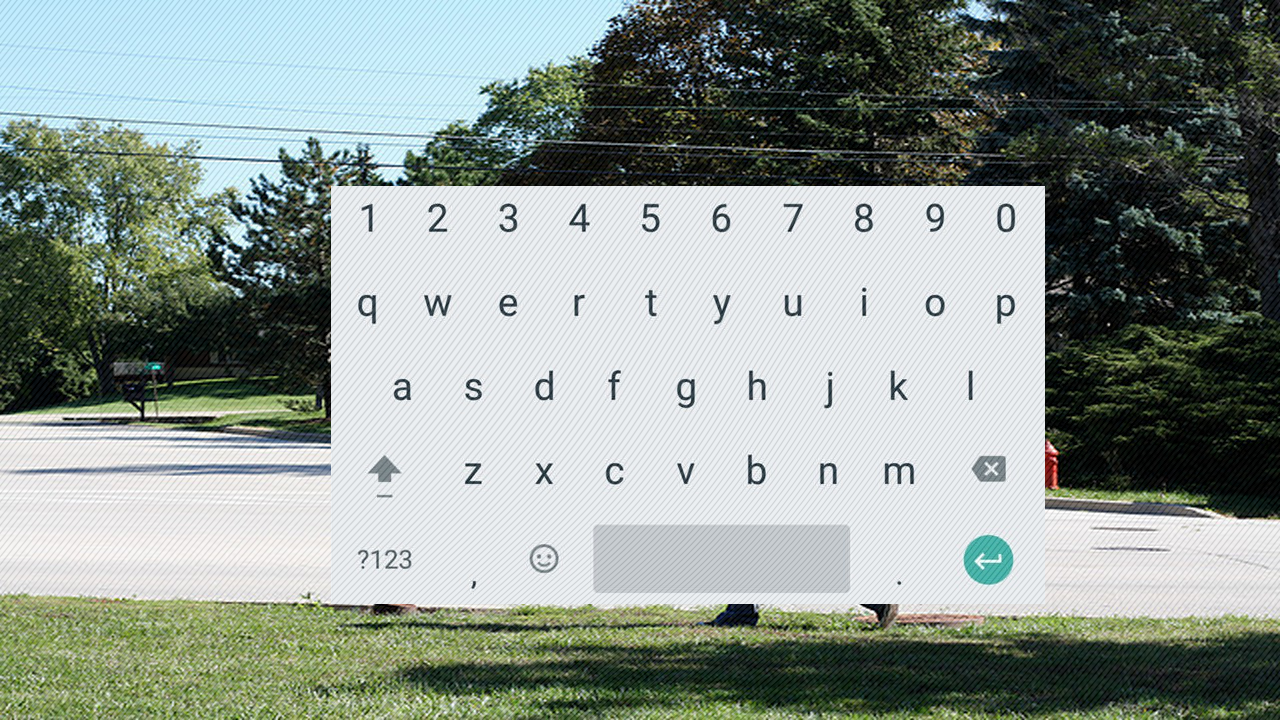
\includegraphics[width=7cm]{img/dataset/keyboard-bg-coco.png} }}
    \qquad
    \subfloat[\centering Average border color as a background]{{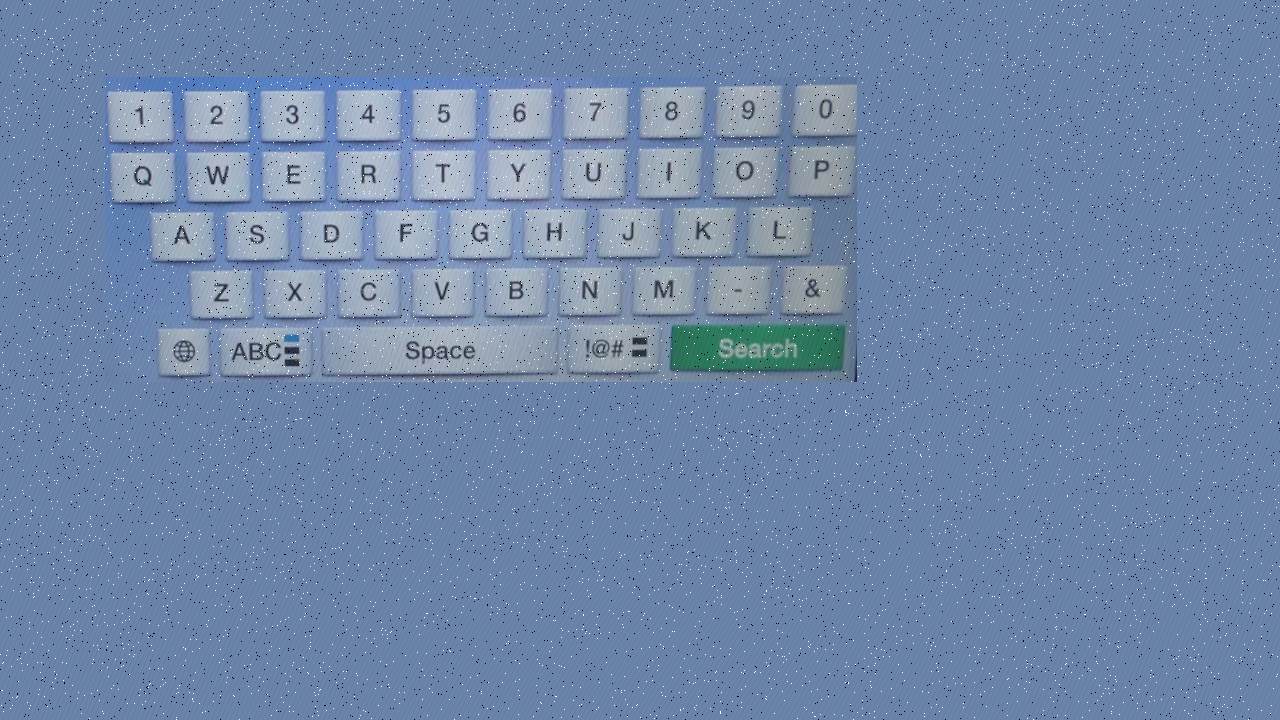
\includegraphics[width=7cm]{img/dataset/keyboard-bg-border.png} }}
    \vspace{-4pt}
    \caption{Comparison of~a COCO image (a) and keyboard border color (b) as~a background shows how the keyboard in~a scene clearly stands out.}
    \label{keyboard-bg-comparison}
\end{figure}

A keyboard is placed on~a background completely randomly. The only constraint is that it cannot overflow. Conditionally, the keyboard can get resized or made transparent and to~the whole image light conditions can be changed or noise added. Moreover, a random moiré effect is always computed as~the images under detection will be screenshots from~a camera. Section~\ref{dataset-keyboards-augmentation} referes about~these modifications in more detail. The whole process summarizes algorithm~\ref{keyboard-generation-algorithm}.

\begin{algorithm}
    \begin{algorithmic}[1]
    \STATE $keyboard\gets get\_keyboard()$
    \IF{$random() \leq 0.25$}
        \STATE $keyboard\gets resize(keyboard, random(0.5, 2))$
    \ENDIF
    \IF{$random() \leq 1/3$}
        \STATE $keyboard\gets make\_transparent(keyboard, random(0.5, 1))$
    \ENDIF
    \STATE $bg\gets get\_background()$
    \STATE $img\gets put\_keyboard\_on\_bg(keyboard, bg)$
    \IF{$random() \leq 0.5$}
        \STATE $img\gets change\_brightness(img)$
    \ENDIF
    \IF{$random() \leq 0.9$}
        \STATE $img\gets add\_random\_noise(img)$
    \ENDIF
    \STATE $img\gets add\_moire(img)$
    \end{algorithmic}
    \caption{Pseudocode for generation of single image for keyboards dataset}
    \label{keyboard-generation-algorithm}
\end{algorithm}

\subsection{Data augmentation}
\label{dataset-keyboards-augmentation}
Owing to~the office or lab conditions in~which AIVA operates, no natural elements like rain need to~be taken into~consideration. Moreover, thanks to~the camera calibration system, other modifications such as rotation or perspective can be omitted. In~the end, only various light conditions, noise and different moiré effects are the real problems. Apart from these, keyboard size and transparency with respect to~the background are also subjected to~the data augmentation process.

If we follow the algorithm~\ref{keyboard-generation-algorithm}, firstly the keyboard is resized. This happens with a~25~\% probability. The image can be changed to~any size in~the range of~twice as small to~twice as~big as~the original. However, boundaries are in~place, so that it cannot overflow the background. Next in~line is the transparency which is applied with probability~\(1/3\) and it is quite simple as the only thing necessary is adding the alpha channel. The alpha is chosen randomly from~interval \(\langle0.5, 1\rangle\). Both of~these modifications are applied directly on~the keyboard region itself, whereas the following augmentation methods concern the whole image.

To~simulate different light conditions, brightness change is applied to~every other image. For~that, gamma correction is used. Firstly, \(\gamma\) is picked from interval \(\langle0.5, 1.5\rangle\) where \(\gamma < 1\) makes the image darker and \(\gamma > 1\) makes it lighter. Secondly, \(\gamma\) is applied to~the image using equation~\ref{equation-gamma}. Image must be normalized from~\(\langle0, 255\rangle\) to~\(\langle0, 1\rangle\) for~the gamma application and than converted back. Figure~\ref{dataset-keyboards-augmentation-gamma} shows the difference between the dark, normal and light images.

\begin{equation}
  \label{equation-gamma}
  Output = \left(\frac{Img}{255}\right)^\frac{1}{\gamma} * 255
\end{equation}

\begin{figure}[tbh]
    \centering
    \subfloat[\centering \(\gamma\) = 0.5]{{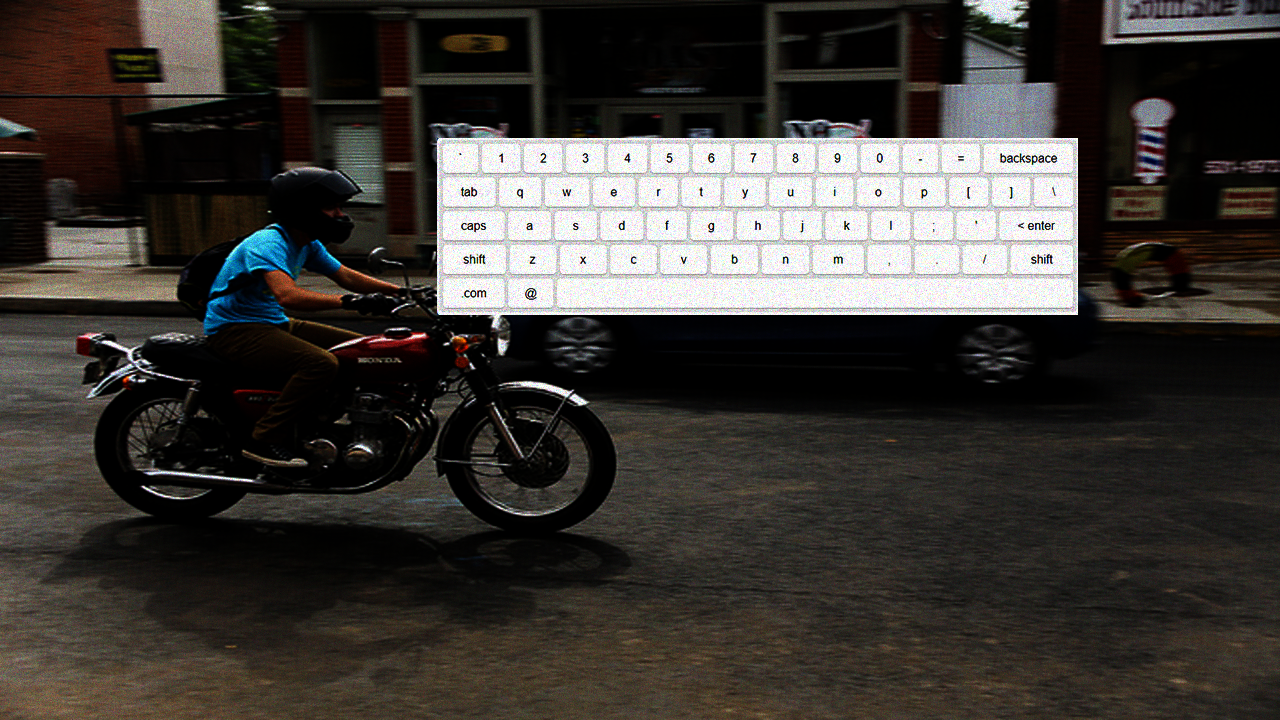
\includegraphics[width=4.95cm]{img/dataset/gamma-dark.png} }}
    \qquad \hspace{-2.34em}
    \subfloat[\centering \(\gamma\) = 1]{{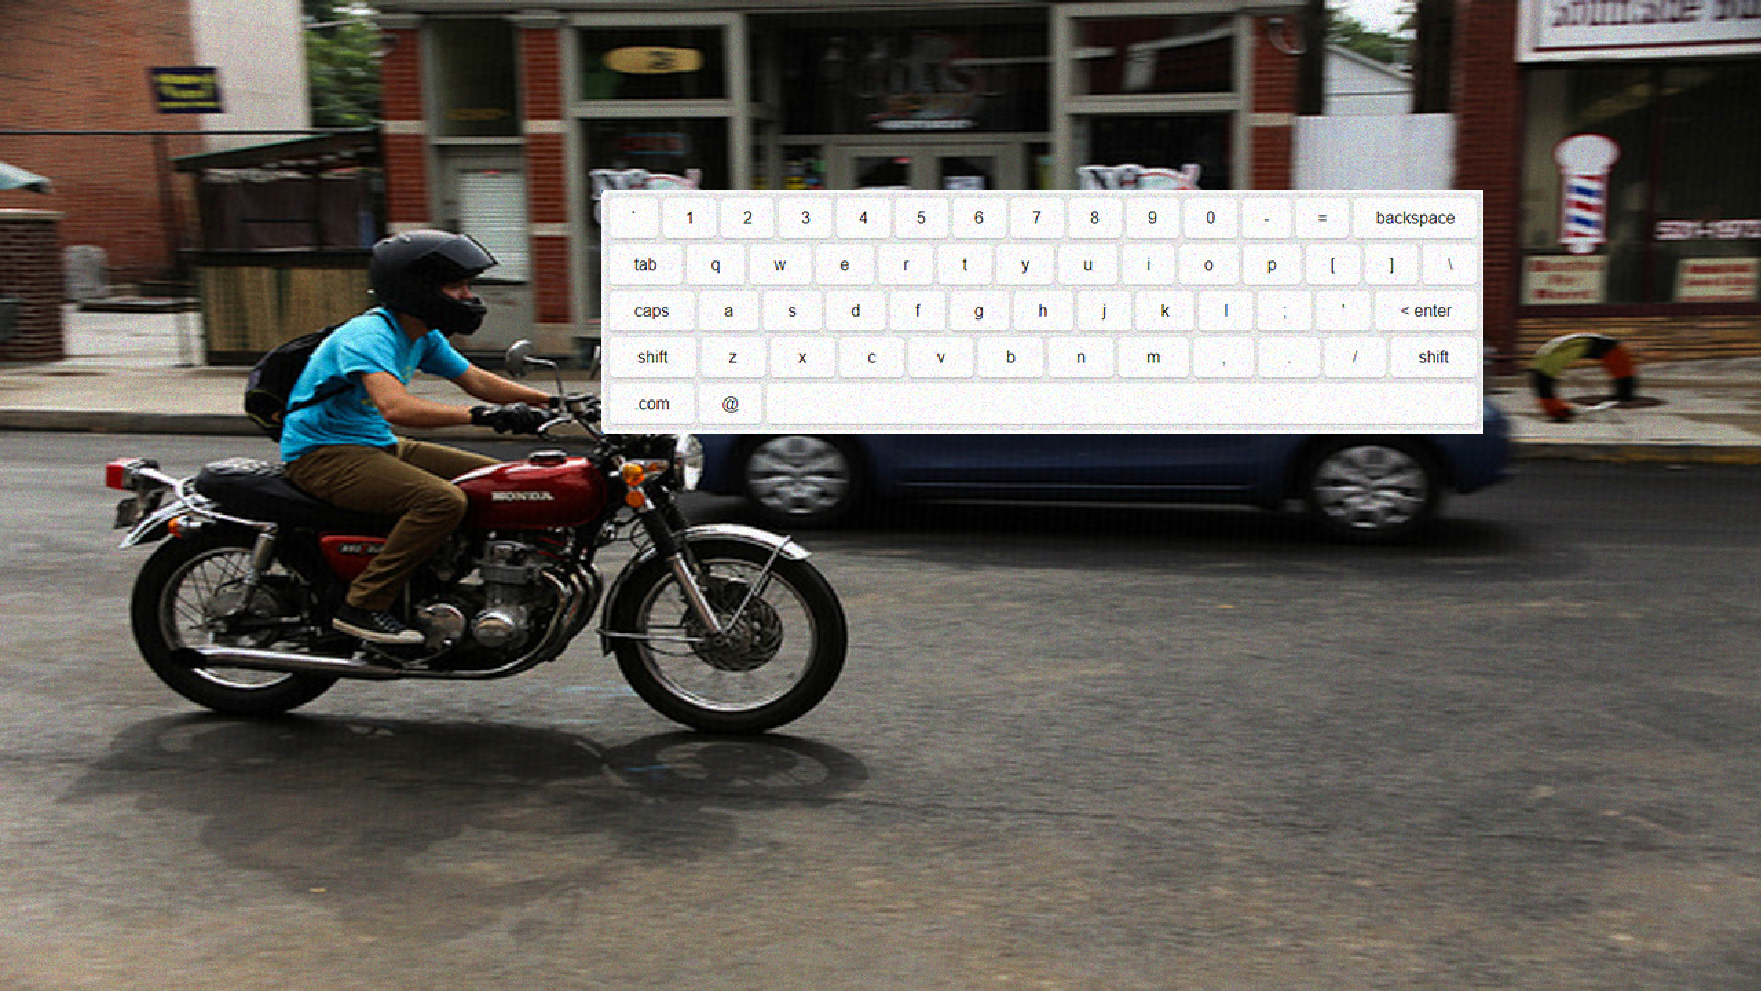
\includegraphics[width=4.95cm]{img/dataset/gamma-normal.pdf} }}
    \qquad \hspace{-2.34em}
    \subfloat[\centering \(\gamma\) = 1.5]{{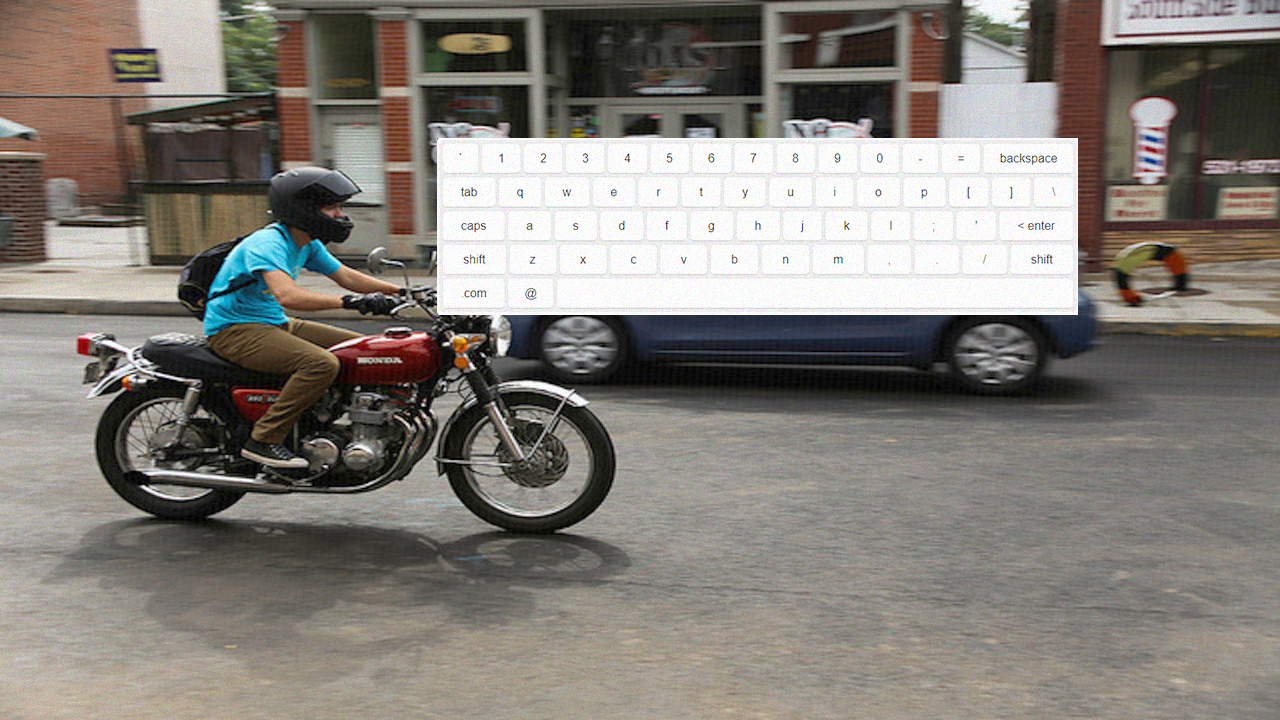
\includegraphics[width=4.95cm]{img/dataset/gamma-light.png} }}
    \caption{Comparison of~dark~(a), original~(b) and light~(c) versions of~an image. The resulting image of~the brightness change application can be anywhere in~between these values. Note that even brighter images would be viable for~most images, however, for~some, it could be too much, so these margins were selected for~both generalization and equal dark/light distribution.}
    \label{dataset-keyboards-augmentation-gamma}
\end{figure}

The next augmentation technique is noise addition. As~noise in an image is quite common, it is generated in~90~\% of them. Four types of~noise with~the same probability of occurrence were used. The first one is Gaussian noise. The Gaussian parameters are set to~\(\mu = 0\) and \(\sigma \in \langle0.5, 10\rangle\)~\ref{equation-gaussian-noise}. The randomly generated noise is then added to~the image.

\begin{equation}
  \label{equation-gaussian-noise}
  Img = Img + N(0, \sigma^2) \hspace{0.5cm} \sigma \in \langle0.5, 10\rangle
\end{equation}

The next one is Poisson noise. This noise makes the image very bright though, so the noise values are randomly divided by~a number from~\{2, 3, 4, 5, 6\} to~reduce its effect~\ref{equation-poisson-noise}.

\begin{equation}
  \label{equation-poisson-noise}
  Img = Img + \frac{Pois(Img)}{r} \hspace{0.5cm} r \in \{2, 3, 4, 5, 6\}
\end{equation}

Another noise is salt and pepper. It iterates through every pixel in~the image and with~a certain probability it sets a pixel to~white or black~\ref{equation-sp-noise}. This probability is again randomly chosen from~interval \(\langle0.005, 0.01\rangle\).

\begin{equation}
  \label{equation-sp-noise}
  Img[i] = \begin{dcases}
 0 & \text{if}\hspace{6pt}r < P
 \\
 255 & \text{if}\hspace{6pt}r > 1 - P
 \\
 Img[i] & \text{else}
 \end{dcases}
 \hspace{0.5cm} r \in \langle0.5, 10\rangle, P \in \langle0.005, 0.01\rangle
\end{equation}

The last one is speckle noise. To~generate such noise, the image is multiplied by~a random map from~the standard normal distribution and optionally can be multiplied by~a variance. The variance is again randomly chosen from~interval \(\langle0.05, 0.4\rangle\) and it controls the noise intensity. In~the end, it is added to~the original image~\ref{equation-speckle-noise}. A~comparison of~these~4~noises is shown in~figure~\ref{dataset-keyboards-augmentation-noise}. 

\begin{equation}
  \label{equation-speckle-noise}
  Img = Img + Img * N(0, 1) * var \hspace{0.5cm} var \in \langle0.05, 0.4\rangle\
\end{equation}

\begin{figure}[tbh]
    \centering
    \subfloat[\centering Gaussian noise]{{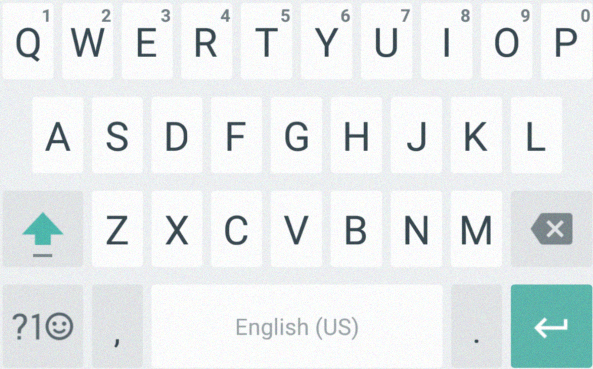
\includegraphics[width=7cm]{img/dataset/noise-gauss.png} }}
    \subfloat[\centering Poisson noise]{{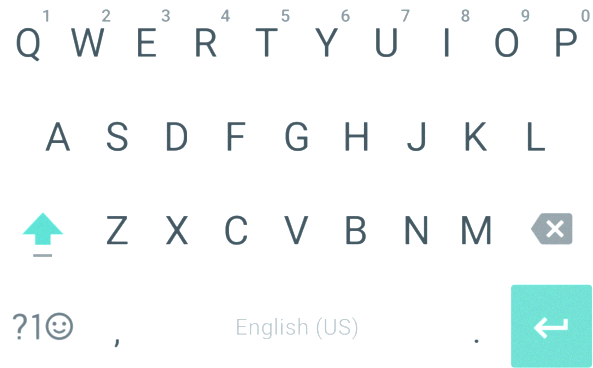
\includegraphics[width=7cm]{img/dataset/noise-poisson.png} }}
    \quad
    \subfloat[\centering Salt and pepper noise]{{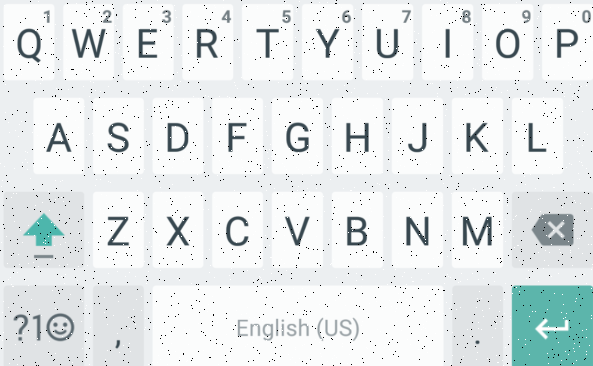
\includegraphics[width=7cm]{img/dataset/noise-sp.png} }}
    \subfloat[\centering Speckle noise]{{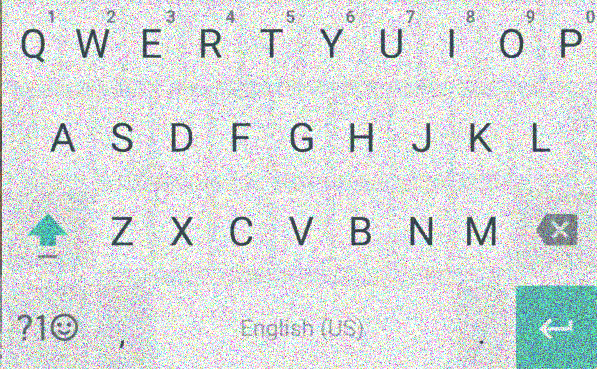
\includegraphics[width=7cm]{img/dataset/noise-speckle.png} }}
    \caption{Comparison of~Gaussian (a), Poisson (b), S\&P (c) and speckle (d) noises}.
    \label{dataset-keyboards-augmentation-noise}
\end{figure}

The final data augmentation method is moiré effect generation. This is particularly \hbox{important} as~the image subjected to~the object detection is usually a target device screen taken by~a camera which tends to~exhibit moiré pattern behaviour. To~create a moiré effect in~an image, python \texttt{latticegen} library~\cite{latticegen} and especially method \texttt{anylattice\_gen(r\_k, theta, order, symmetry)} was used. It is capable of~creating parameterized moiré lattices. To~set the lattice scale (how big or seemingly zoomed the lattice is) there is \texttt{r\_k} \hbox{parameter} which I select randomly from interval \(\langle0.01, 0.25\rangle\). Parameter \texttt{theta} stands~for~\hbox{lattice} \hbox{rotation} and it can be anything between~0 and~90~degree angle. The \texttt{order} parameter is for~simplicity described as \say{The higher the order, the more well-resolved the atoms are as~single spots}~\cite{latticegen} which can be seen in~figure~\ref{latticegen-order}. One of~the first~3 orders is randomly chosen for~the generation.

\begin{figure}[hbt]
    \centering
    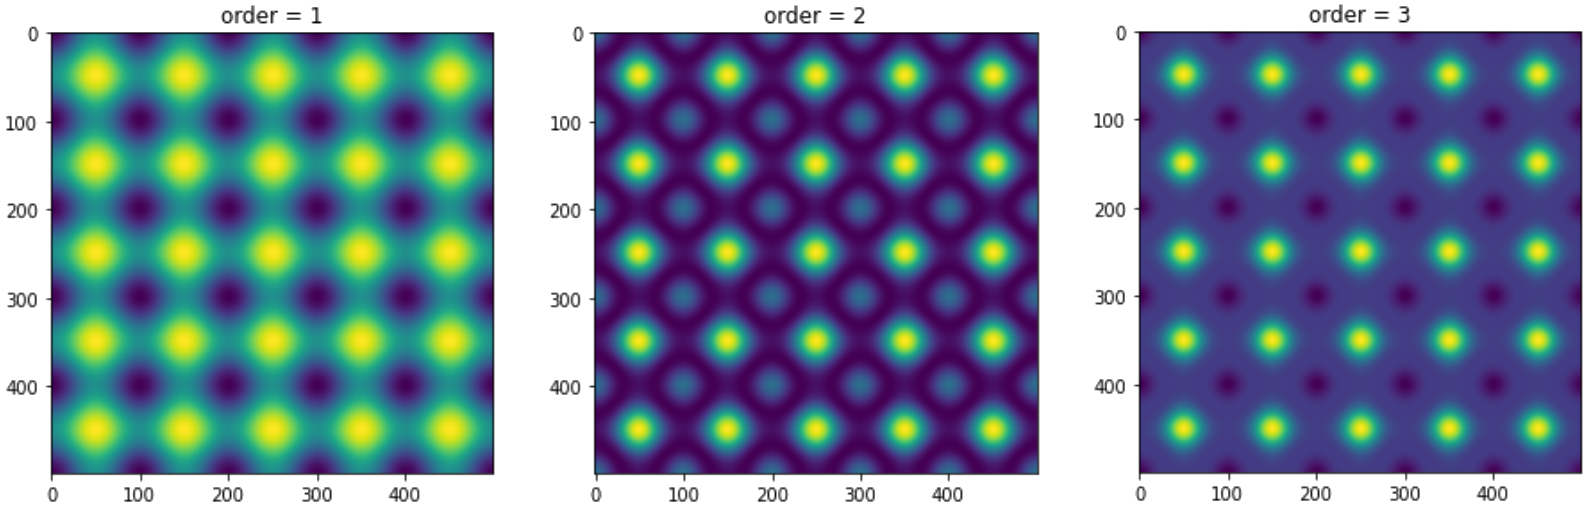
\includegraphics[width=0.98\textwidth]{img/dataset/latticegen-order.png}
    \caption{Different latticegen orders (adapted from~\cite{latticegen})}
    \label{latticegen-order}
\end{figure}

The last parameter \texttt{symmetry} controls the shape of~the spots. The most common moiré effect on~screens seems to~be lines which correspond to~symmetry value~1. For~that reason, the value~1 is chosen in~50~\% of~cases. The rest is equally distributed to~values \{2, 3, 4, 5\}. Different symmetries depicts figure~\ref{latticegen-symmetry}.

\begin{figure}[hbt]
    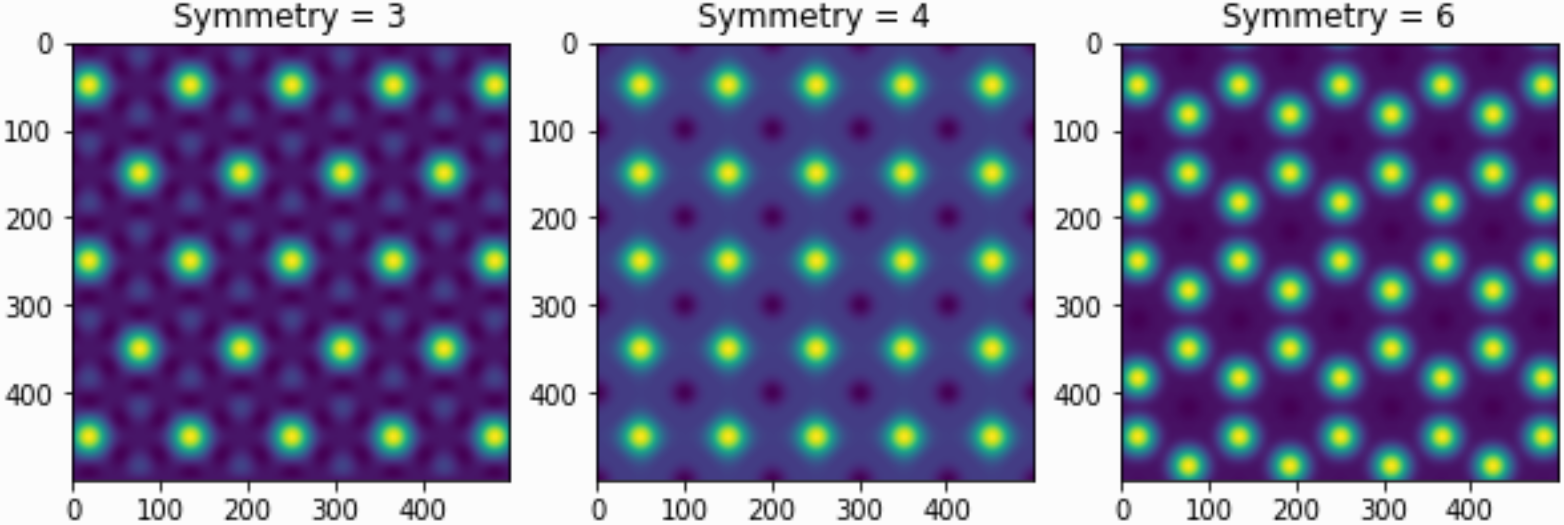
\includegraphics[width=1\textwidth]{img/dataset/latticegen-symmetry.png}
    \caption{Different latticegen symmetries (taken from~\cite{latticegen})}
    \label{latticegen-symmetry}
\end{figure}

So that the lattice is not always regular, a shift taken from the library is applied. For~the shift, no further randomization is done as~it behaves differently on~various lattice designs. To~deform the regularity even more, several lattices can be combined together. In~the end, either a single lattice or a combination of~2 lattices is used with equal probability.

\section{Characters}
\label{dataset-characters}
In~many ways, the generation of~characters dataset is the same as~the one for~the keyboards. Some characters are selected, put on~a background and then noise and moiré effect are added. Noise is created similarly as~to the keyboard images. The only difference is that additional gaussian noise is added with 50~\% probability. Concerning the moiré effect, the lattice is always of the first order and the symmetry is always~1 (lines) as~the special patterns empirically did not influence the image much. Gamma correction is omitted because the characters dataset is in~grayscale, so the brightness naturally differs simply by~choosing different gray colors. There are several reasons for~grayscale images. The most important one is that the keyboards are very contrastive. By converting to~grayscale, the characters will always be light on~a dark background or vice versa no matter the original color design. Another reason is that processing a grayscale image is easier than a colored one. In~addition, to~simulate bad-quality images, every third image is blurred by~scaling down (randomly up to half) and up again. The algorithm~\ref{characters-generation-algorithm} demonstrates the process.

\begin{algorithm}
    \begin{algorithmic}[1]
    \STATE $char\gets select\_character()$
    \STATE $bg\gets generate\_background()$
    \STATE $img\gets put\_characters\_on\_bg(char, bg)$
    \IF{$random() \leq 0.5$}
        \STATE $img\gets add\_gaussian\_noise(img)$
    \ENDIF
    \IF{$random() \leq 0.95$}
        \STATE $img\gets add\_random\_noise(img)$
    \ENDIF
    \STATE $img\gets add\_moire(img)$
    \IF{$random() \leq 1/3$}
        \STATE $img\gets blur(img)$
    \ENDIF
    \end{algorithmic}
    \caption{Pseudocode for generation of single image for characters dataset}
    \label{characters-generation-algorithm}
\end{algorithm}

Having described the high level differences to~the keyboards dataset generation, the rest of~this section focuses on~the selection and placement of~the characters on~the background. The set of~characters consists of~alphanumeric ones (a-zA-Z0-9), special characters from the sequence .,:;'"?!@\#\$£€\%\^{ }\&()\{\}[]<>/\textbackslash\_+-*÷= and icons for~backspace, shift, enter, space and tab. These are repeatedly iterated during the dataset generation. For~further reference, an iteration's current character is considered to~be the \say{main character}. The background on~which the characters are placed is created as~follows. The resolution is set to 640x640 for several reasons. A keyboard usually takes around~\(1/2\) of~the screen's height so the target resolution~1920x1020 is covered. Moreover, object detectors take square images and the current state-of-the art YOLOv7 uses 640x640. Furthermore, the objective is to find characters of different but bounded sizes, so the background resolution does not play a significant role anyway. As~for~the background color, it is usually light or dark. The background color probability is shifted towards such pixel intensities on~the gray scale according to~the formula~\ref{equation-bg-grayscale}.

\begin{equation}
  \label{equation-bg-grayscale}
  bg\_color = \begin{dcases}
 randInt(0, t) & \text{if}\hspace{6pt}r \leq \frac{1}{3}
 \\
 randInt(255 - t, 255) & \text{if}\hspace{6pt}r \in (\frac{1}{3}, \frac{2}{3}\rangle
 \\
 randInt(0, 255) & \text{else}
 \end{dcases}
 \hspace{0.5cm} r \in \langle0, 1\rangle, t = 64
\end{equation}

A convenient threshold \(t\) for~the light/dark boundaries appeared to~be value~64. The formula~\ref{equation-bg-grayscale} basically says that with~a~\(1/3\) chance the background color will be dark, with~another~\(1/3\) chance that light or else it will be completely random.

The placement of~characters on~a background is a bit more complicated. The main character is rendered several times on the background and other random characters with~it. Different position, color and font, which includes font family, size, weight and style, are selected for~each character. To~solve the position selection, an attempt to~just randomly put characters on~the background and check for~intersections was made in~the beginning. However, the intersections occurred so often that too few characters could be safely rendered which left a lot of~free space. As~a consequence, a grid system was devised. The largest font size used is~64 which means that after dividing the resolution, from which a random padding is subtracted so that the characters are not directly on~a border, a~9x9 grid is created. In~order to render not only individual characters but words as~well, one or~two lines are randomly left out of~the grid for~word generations. This is because a detector might otherwise not learn to~recognize characters in~the proximity of~other characters. The generated words are either keyboard special words (space, shift, enter...), mode-changing sequences (abc, ?123, \#+=...) or completely random character sequences. Out of~the remaining (7|8)x9~=~63-72 grid cells, a quarter to~half is randomly taken by the main character and another quarter to~half by~other random characters. As~a result, there is no intersection and even the grid is not that apparent as~not all grid cells are utilised and different characters of~various fonts and sizes are rendered.

Concerning the color selection, the contrast between the characters and keyboard/key background is usually very high, often even black on~white and vice versa. Thus, a pixel intensity threshold for~the difference between the background and a character color can be set. The formula~\ref{equation-font-color} demonstrates the calculation of~available colors to~be randomly chosen from, where \(I_{bg}\) is the intensity of~the background pixels and \(t\) stands for~the threshold. In~75~\% of~cases, the threshold value is~92 due to~the high contrasts and~24 otherwise so~that even unusual low contrastive keyboards can be learned. The visual difference between the threshold pixel intensities with respect to~different backgrounds provides figure~\ref{font-color-selection}.

\begin{equation}
  \label{equation-font-color}
  available\_colors = \langle0, 255\rangle \setminus \langle I_{bg} - t, I_{bg} + t\rangle \hspace{0.5cm} t \in \{24, 92\}
\end{equation}

\begin{figure}[tbh]
    \centering
    \subfloat[\centering I(24) on I(0)]{{
\includegraphics[width=3.5cm]{img/dataset/font-color-dark-light-24.png} }}
    \subfloat[\centering I(92) on I(0)]{{
\includegraphics[width=3.5cm]{img/dataset/font-color-dark-light-92.png} }}
    \subfloat[\centering I(255-24) on I(255)]{{
\includegraphics[width=3.5cm]{img/dataset/font-color-light-dark-24.png} }}
    \subfloat[\centering I(255-92) on I(255)]{{
\includegraphics[width=3.5cm]{img/dataset/font-color-light-dark-92.png} }}
    \\[-6pt]
    \subfloat[\centering I(128-24) on I(128)]{{
\includegraphics[width=3.5cm]{img/dataset/font-color-middle-dark-24.png} }}
    \subfloat[\centering I(128-92) on I(128)]{{
\includegraphics[width=3.5cm]{img/dataset/font-color-middle-dark-92.png} }}
    \subfloat[\centering I(128+24) on I(128)]{{
\includegraphics[width=3.5cm]{img/dataset/font-color-middle-light-24.png} }}
    \subfloat[\centering I(128+92) on I(128)]{{
\includegraphics[width=3.5cm]{img/dataset/font-color-middle-light-92.png} }}
    \caption{The first row shows~24 and~92 pixel intensity I(x) differences on~a black/white background. The second row depicts the same for~a middle gray background bidirectionally.}
    \label{font-color-selection}
\end{figure}

With~regards to~the font selection, 46~different font families such as~Calibri, Arial, Verdana etc. are used. For~most of~them, bold and italic versions are available. As~italic characters are quite uncommon on~keyboards, the normal to~italic ratio is~95:5. On~the other hand, bold characters are seen more often, so a bold font is used in~40~\% of~cases instead~of the regular one. Font size is selected from~interval \(\langle8, 64\rangle\) with~a~50~\% chance of~inclination towards the lower half.

As~there are several characters in~an image, the annotation file format needed to~be changed. Like in~the keyboards annotation, the dictionary key is a filename, however, the value is not a single bounding box for~a single keyboard in~an image, but another dictionary for~characters. In~the value dictionary, keys are individual characters and values are lists of~bounding boxes as~figure~\ref{characters-annotation-json} shows.

Totally, 40~000 character images are generated with train-validation-test ratio~70:20:10 and an example is shown in figure~\ref{dataset-characters-image}. In~the training set, there are 2~287~613 characters. As~there are~99 of~target classes, each one has on~average~23~107 representations. This is significantly more than my Amazon counterparts who manually annotated characters on~634~keyboards~\cite{amazon-paper}. As~they work with~68~characters and~26~(a-z~vs~A-Z) are usually mutually exclusive, there could be a maximum of~42~characters in~each image which results in 634x42=26~628 characters. If uniform distribution of~characters is presumed, it makes 26~628/68=391 samples for~each character. However, from~my findings lowercase characters are more usual in~internet keyboard images, so the uniform distribution is doubtful. The benefits of~my dataset are the following:

\begin{itemize}[topsep=0pt,itemsep=-1.5pt,partopsep=6pt]
    \item There is substantially more samples for~each character.
    \item Any character can be generated, not just what is found in~an internet image.
    \item Characters are generated uniformly, none has significantly more samples than others.
    \item There is no need for~manual annotation.
\end{itemize}

\vspace{-6pt}
\begin{figure}[!hbt]
    \centering
    \begin{boxedverbatim}
"27.png": {
    "A": [
        [463, 193, 491, 223],
        [95, 105, 126, 132],
        [3, 382, 36, 415],
        ...
    ],
    "n": [
        [463, 115, 510, 161],
        [279, 380, 310, 427]
    ],
    ...
},
"28.png": {
    ...
},
...
\end{boxedverbatim}
    \vspace{-6pt}
    \caption{Characters annotation file is a JSON dictionary with a filename as~a key and a dictionary of character~bounding boxes in~format [x1, y1, x2, y2] as~a value.}
    \label{characters-annotation-json}
\end{figure}

\vspace{-12pt}
\begin{figure}[!hbt]
    \centering
    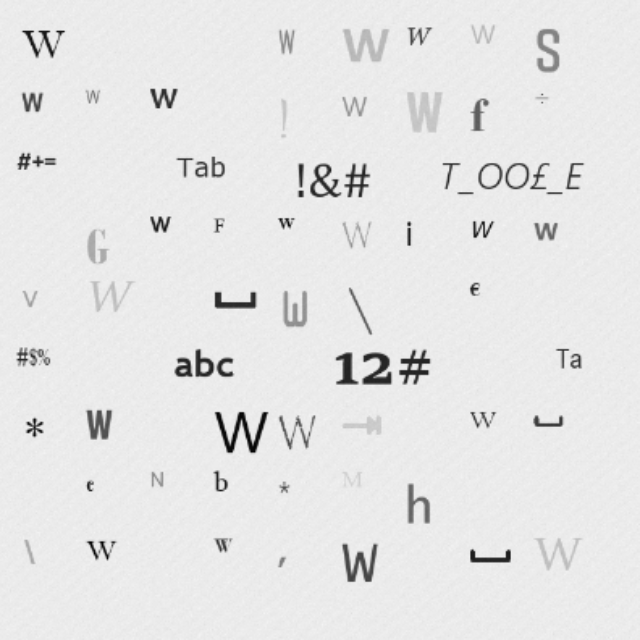
\includegraphics[width=0.66\textwidth]{img/dataset/characters-img-W.png}
    \vspace{-6pt}
    \caption{An image from characters dataset with W as~the main character}
    \label{dataset-characters-image}
\end{figure}

\section{Post-processing}
\label{dataset-postprocessing}

In~comparison with~the previous ones, the post-processing dataset serves only for~validation and is substantially smaller. There are~2~major issues which need to~be solved after the actual detection. The first one is that a lot~of times more than one character is written on~a key. On~a physical keyboard, the other character(s) is usually accessed by~switching keyboard language or by~pressing the shift key. On~digital keyboards, they mostly just foreshadow what special character is in~another keyboard mode. For~my problem, only the main keyboard character is relevant as~AIVA's robotic arm cannot press multiple buttons. Therefore, these other characters need to~be recognized and discarded based on~the keyboard layout. The second issue is that not all characters will necessarily be detected or recognized correctly e.g.~'o'~vs~'O'~vs~'0'. This needs to~be solved in~post-processing and a proper validation dataset must be provided for~such a task.

From~the collected keyboard regions,~120~which are appropriate to~test these issues are selected. These are further split 50:50 into~2~groups. The first group is called \emph{layout} and it validates the correct detection of~characters on~different keyboard layouts, including the omission of~unwanted characters. The second one is named \emph{missing\_chars} where not only single characters but also sequences of~characters are removed to~test if they can be automatically computed. Moreover, even characters in keywords (e.g.~\emph{space}) are left out~to~test partial recognition of~keywords for~special keys.
